\documentclass[12pt]{article}
\usepackage{a4wide}
\usepackage{amsmath,amssymb}
\usepackage{bm}
\usepackage[colorlinks]{hyperref}
\usepackage{listings}
\usepackage{graphicx}


\begin{document}

\title{Report V1}
\author{}
\maketitle



\tableofcontents

\section{Introduction}

Dans ce projet, on s’intéresse à un problème elliptique (
une équation de diffusion en une ou deux dimensions d’espace) où le coefficient de diffusion
dépend d’un paramètre, et on suppose qu’on a besoin de résoudre le problème pour un nombre
important de valeurs de ce paramètre.

Voici  l'équation différentielle :
$$
\begin{cases} 
- \frac{d }{dx}(D(x)\frac{\partial u}{\partial x}) + u(x) = f(x) , x \in \Omega \\
u = 0 , x \in \partial \Omega \\
D(x) = 
\begin{cases} 
1 , x \in \Omega _{1} \\
\mu , x \in \Omega _{2}
\end{cases}
\end{cases}
$$



Dans ce contexte, résoudre un nombre important de fois le problème elliptique (par la méthode des éléments finis par exemple) devient extrêmement onéreux. Le principe de la méthode des bases réduites est de procéder à ces
évaluations en deux temps : (1) on résout d’abord le problème elliptique
(par la méthode de éléments finis) pour un nombre relativement modeste
de valeurs du paramètre, puis (2) on utilise les solutions ainsi obtenues pour
engendrer un espace vectoriel de dimension réduite où l’on cherchera une
approximation de la solution du problème elliptique pour toutes les autres
valeurs du paramètre .

Comment choisir les quelques solutions de base ? Nous utiliserons l'algorithme glouton
qui procède de  la manière suivante :  

$$
\begin{cases} 
B_n = {\vec{u_1},\vec{u_2} , ... ,\vec{u_n}}  \\
\vec{u_{n+1}} =  argmax(\Delta(\mu) ) , \text{ avec  }  \Delta(\mu) = || u(\mu) - P_{B_n}(u)|| \\
B_{n+1} = {\vec{u_1},\vec{u_2} , ... ,\vec{u_n},\vec{u_{n+1}} } \\
\end{cases}
$$

Comme le calcul de $ \vec{u_{n+1}} $ est  assez long , Pour palier ce problème, nous
envisagerons de d'utiliser des réseaux de neuronnes pour construire $ \Delta(\mu) $.

\section{Méthode des Elements finis}



\subsection{Formulation Variationnelle}

$$
\begin{cases} 
- \frac{d }{dx}(D(x)\frac{\partial u}{\partial x}) + u(x) = f(x) , x \in \Omega \\
u = 0 , x \in \partial \Omega \\
D(x) = 
\begin{cases} 
1 , x \in \Omega _{1} \\
\mu , x \in \Omega _{2}
\end{cases}
\end{cases}
$$

$
\text{Avec } \Omega =  ]0,1[ , 
$

$
\Omega _{2} = ]0.19; 0.21[ \text{U} ]0.39; 0.41[ \text{U} ]0.59; 0.61[ \text{U}]0.79; 0.81[ , \text{et }  \Omega _{1} = \Omega \backslash\ \Omega_{2} 
$


$$
\forall x \in \Omega , 
-(D(x)u'(x))' + u(x) = f(x) 
$$
$$\Longleftrightarrow $$ 

$$
\forall v \in H_{0}^{1}(\Omega) ,  
-v(x)-(D(x)u'(x))' + v(x)u(x) =  v(x)f(x) 
$$

$$\Longleftrightarrow $$ 

$$
\int_{\Omega} -v(x)-(D(x)u'(x))' + \int_{\Omega} v(x)u(x)
= 
\int_{\Omega} v(x)f(x)
$$

$$\Longleftrightarrow$$

$$
\int_{\Omega} D(x)v'(x)u'(x)dx + \int_{\partial \Omega} D(x)v(x)u'(x) + \int_{\Omega} v(x)u(x) \\
$$
$$
=  \int_{\Omega} D(x)v'(x)u'(x) + \int_{\Omega} v(x)u(x) \\
= \int_{\Omega} 1_{\Omega_{1}}v'(x)u'(x) + \int_{\Omega} 1_{\Omega_{2}}\mu v'(x)u'(x) + \int_{\Omega} v(x)u(x) \\
$$
$$
= \int_{\Omega} 1_{\Omega_{1}}v'u' + \int_{\Omega} 1_{\Omega_{2}}\mu v'u' + \int_{\Omega} vu 
$$


On pose alors ceci :

$$
\alpha _ {\mu}(u,v) 
= \int_{\Omega} 1_{\Omega_{1}}v'u' + \mu\int_{\Omega} 1_{\Omega_{2}} v'u' + \int_{\Omega} vu \\
l(v) = \int_{\Omega} f(x)v(x)
$$

Et la formulation variationnelle devient
$$
\alpha _ {\mu}(u,v) = l(v) ,  \forall v \in H_{0}^{1}(\Omega) 
$$



\subsection{Construction de l’espace d’approximation } 

\subsubsection{ Notations}

Maillage : $x_{min} = x_0 < x_1 < .... < x_{N-1} < x_N = x_{max}$ 

\noindent Nombre d'éléments (mailles) : $N$

\noindent Nombre de noeuds : $N+1$

\noindent Nombre de noeuds internes : $N-1$

\noindent Tailles de mailles : $h_j = x_{j+1} - x_j$   et   $h_j = a_{j+1} - a_j$

\noindent On pose :  K = \{a,b\} , $ \Sigma = \{a,b\} $ , $P = P_{1}(\mathbb{R}) = \{ p = \alpha + \beta x \}$


\noindent $\Omega = \Omega_{1} \cup \Omega_{2} $ , avec $\Omega_{1} = \bigcup _{i =1} ^{N} [x_{i},x_{i+1}] $ , et  $\Omega_{2} = \bigcup _{i =1} ^{N} [a_{i},a_{i+1}] $

\noindent Espace d'aprproximation : $ V_{h} = \{ v_{h} \in C^{0} : v_{h}|\Gamma = 0 , 
v_{h}|K \in P_{1}(K)\}$ , Avec $ V_{h}\subset H_{0}^{1}(\Omega)  $






\subsubsection{Construction des fonctions de base } 

Support des  fonctions de bases $\varphi_{i} $: $ [{x}_{i-1},{x}_{i+1}]$.

\noindent Définitions des fonctions de bases : 

$$
\varphi_{i} (x_{j}) = \delta_ {ij} , \forall i,j = 1,...,N
$$


$$
\forall i \in [1,N], 
\varphi_{i} (x) = 
\begin{cases}
\frac{ x-x_{i-1} }{h_{i}} , x \in [x_{i-1},x_{i}[\\
-\frac{ x-x_{i+1} }{h_{i+1} } , x \in ]x_{i},x_{i+1}]  \\
1 , x =  x_{i} \\
0 , \text{ sinon }
\end{cases}
$$


\noindent Et sa dérivée :

$$
\forall i \in [1,N], 
\varphi_{i}'(x) = 
\begin{cases}
\frac{1}{h_{i}} , x \in [x_{i-1},x_{i}[ \\
-\frac{1}{h_{i+1}} , x \in ]x_{i},x_{i+1}]  \\
0 , sinon 
\end{cases}
$$



%---- mettre image fonction de base phi_i,phi_i-1,phi_i+1


\begin{figure}[h]
\begin{center}
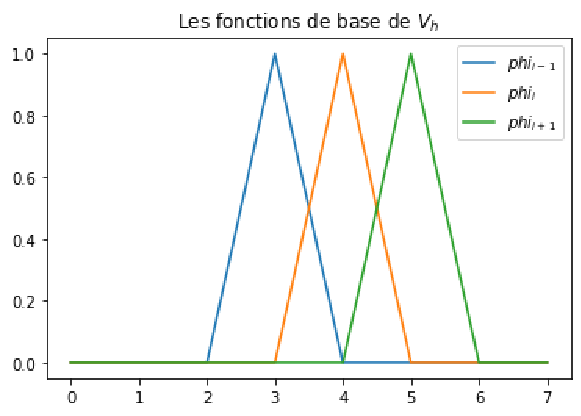
\includegraphics[scale=1]{fct_baseVh.pdf}
\caption[]{Illustraton des fonction de base}
\end{center}
\end{figure}




\subsection {Construction des Matrices éléments finis}


$$
A_{ij} = a_{\mu}(\varphi _{i} ,\varphi _{j})   
= \int_{\Omega} 1_{\Omega_{1}} \varphi'_{i} \varphi'_{j} + \mu \int_{\Omega}  1_{\Omega_{2}} \varphi'_{i}\varphi'_{j} + \int_{\Omega} \varphi _{i} \varphi_{j}  
$$ 
$$
\text{En posant }  A_{1} = \int_{\Omega} 1_{\Omega_{1}} \varphi'_{i} \varphi'_{j}    \text{ ,  } A_{2} =
\int_{\Omega} 1_{\Omega_{2}} \varphi'_{i} \varphi'_{j} \text{  et  }  M = \int_{\Omega}
\varphi_{i} \varphi_{j}
$$



$$
(A_{1})_{ij} = 
\begin{cases}
a(\varphi_{i},\varphi_{j}) = 0 ,    |(i-j)| \ge 2 \\
a(\varphi_{i},\varphi_{i+1}) =  \int_{\Omega_{1}} \varphi'_{i} \varphi'_{i+1} \\
a(\varphi_{i},\varphi_{i-1}) = \int_{\Omega_{1}} \varphi'_{i} \varphi'_{i-1}  \\
a(\varphi_{i},\varphi_{i}) = \int_{\Omega_{1}}  {\varphi'_{i}}^2   \\
\end{cases}
$$


Sur chaque sous-intervalle de $ \Omega_{1}$ on a :

$$
(A_{1})_{ij} = 
\begin{cases}
a(\varphi_{i},\varphi_{j}) = 0 ,    |(i-j)| \ge 2 \\
a(\varphi_{i},\varphi_{i+1}) = \int_{x_{i-1}}^{x_{i+1}} \varphi'_{i} \varphi'_{i+1} \\
a(\varphi_{i},\varphi_{i-1}) = \int_{x_{i-1}}^{x_{i+1}} \varphi'_{i} \varphi'_{i-1}  \\
a(\varphi_{i},\varphi_{i}) = \int_{x_{i-1}}^{x_{i+1}}  {\varphi'_{i}}^2   \\
\end{cases}
$$

$$
(A_{1})_{ij} = 
\begin{cases}
a(\varphi_{i},\varphi_{j}) = 0 ,    |(i-j)| \ge 2 \\
a(\varphi_{i},\varphi_{i+1}) = 
\int_{x_{i-1}}^{x_{i}} \varphi'_{i} \varphi'_{i+1} + \int_{x_{i}}^{x_{i+1}} \varphi'_{i} \varphi'_{i+1}  \\
a(\varphi_{i},\varphi_{i-1}) = 
\int_{x_{i-1}}^{x_{i}} \varphi'_{i} \varphi'_{i-1} + \int_{x_{i}}^{x_{i+1}} \varphi'_{i} \varphi'_{i-1}  \\
a(\varphi_{i},\varphi_{i}) = 
\int_{x_{i-1}}^{x_{i}}  {\varphi'_{i}}^2 +  \int_{x_{i}}^{x_{i+1}}  {\varphi'_{i}}^2\\
\end{cases}
$$


$$
(A_{1})_{ij} = 
\begin{cases}
a(\varphi_{i},\varphi_{j}) = 0 ,    |(i-j)| \ge 2 \\
a(\varphi_{i},\varphi_{i+1}) = 
\int_{x_{i-1}}^{x_{i}} \frac{1}{h_{i}} *0 + \int_{x_{i}}^{x_{i+1}} -\frac{1}{h_{i+1}}\frac{1}{h_{i+1}}  \\
a(\varphi_{i},\varphi_{i-1}) = 
-\int_{x_{i-1}}^{x_{i}} \frac{1}{h_{i}} *\frac{1}{h_{i}} + \int_{x_{i}}^{x_{i+1}} -\frac{1}{h_{i+1}}*0  \\
a(\varphi_{i},\varphi_{i}) = 
\int_{x_{i-1}}^{x_{i}} \frac{1}{h_{i}} *\frac{1}{h_{i}} + \int_{x_{i}}^{x_{i+1}} \frac{1}{h_{i+1}} *\frac{1}{h_{i+1}} \\
\end{cases}
$$




$$
(A_{1})_{ij} = 
\begin{cases}
a(\varphi_{i},\varphi_{j}) = 0 ,  x \notin [x_{i-1},x_{i+1}]  \\
a(\varphi_{i},\varphi_{i+1}) = -\frac{1}{h_{i+1}}  , x \in [x_{i},x_{i+1}] \\
a(\varphi_{i},\varphi_{i-1}) = -\frac{1}{h_{i}} , x \in [x_{i-1},x_{i}] \\
a(\varphi_{i},\varphi_{i}) =  \frac{1}{h_{i}}*1_{[x_{i-1},x_{i}]} + \frac{1}
{h_{i+1}}*1_{[x_{i},x_{i+1}]} 
\end{cases}
$$

De  même pour $ A_{2} $ on a ceci :

$$
(A_{2})_{ij} = 
\begin{cases}
a(\varphi_{i},\varphi_{j}) = 0 ,    x \notin [x_{i-1},x_{i+1}]  \\
a(\varphi_{i},\varphi_{i+1}) = -\frac{1}{h_{i+1}}  , x \in [x_{i},x_{i+1}] \\
a(\varphi_{i},\varphi_{i-1}) = -\frac{1}{h_{i}} , x \in [x_{i-1},x_{i}] \\
a(\varphi_{i},\varphi_{i}) =  \frac{1}{h_{i}}*1_{[x_{i-1},x_{i}]} + \frac{1}
{h_{i+1}}*1_{[x_{i},x_{i+1}]} 
\end{cases}
$$



$$
(M)_{ij} = 
\begin{cases}
a(\varphi_{i},\varphi_{j}) = 0 ,    |(i-j)| \ge 2 \\
a(\varphi_{i},\varphi_{i+1}) =  \int_{\Omega} \varphi _{i} \varphi _{i+1} \\
a(\varphi_{i},\varphi_{i-1}) = \int_{\Omega} \varphi _{i} \varphi_{i-1}  \\
a(\varphi_{i},\varphi_{i}) = \int_{\Omega}  {\varphi _{i}}^2   \\
\end{cases}
$$

$$
(M)_{ij} = 
\begin{cases}
a(\varphi_{i},\varphi_{j}) = 0 ,    |(i-j)| \ge 2 \\
a(\varphi_{i},\varphi_{i+1}) = \int_{x_{i-1}}^{x_{i+1}} \varphi _{i} \varphi _{i+1} \\
a(\varphi_{i},\varphi_{i-1}) = \int_{x_{i-1}}^{x_{i+1}} \varphi _{i} \varphi _{i-1}  \\
a(\varphi_{i},\varphi_{i}) = \int_{x_{i-1}}^{x_{i+1}}  {\varphi _{i}}^2   \\
\end{cases}
$$

$$
(M)_{ij} = 
\begin{cases}
a(\varphi_{i},\varphi_{j}) = 0 ,    |(i-j)| \ge 2 \\
a(\varphi_{i},\varphi_{i+1}) = 
\int_{x_{i-1}}^{x_{i}} \varphi _{i} \varphi _{i+1} + \int_{x_{i}}^{x_{i+1}} \varphi _{i} \varphi _{i+1}  \\
a(\varphi_{i},\varphi_{i-1}) = 
\int_{x_{i-1}}^{x_{i}} \varphi _{i} \varphi _{i-1} + \int_{x_{i}}^{x_{i+1}} \varphi _{i} \varphi _{i-1}  \\
a(\varphi_{i},\varphi_{i}) = 
\int_{x_{i-1}}^{x_{i}}  {\varphi _{i}}^2 +  \int_{x_{i}}^{x_{i+1}}  {\varphi _{i}}^2\\
\end{cases}
$$



$$
(M)_{ij} = 
\begin{cases}
a(\varphi_{i},\varphi_{j}) = 0 ,    |(i-j)| \ge 2 \\
a(\varphi_{i},\varphi_{i+1}) =  
\int_{x_{i-1}}^{x_{i}} \frac{x-x_{i-1}}{h_{i}}*0  -\int_{x_{i}}^{x_{i+1}} \frac{x-x_{i+1}}{h_{i+1}}\frac{x-x_{i}}{h_{i+1}}  \\
a(\varphi_{i},\varphi_{i-1}) = 
-\int_{x_{i-1}}^{x_{i}} \frac{x-x_{i-1}}{h_{i}}\frac{x-x_{i}}{h_{i}}  -\int_{x_{i}}^{x_{i+1}}\frac{x-x_{i+1}}{h_{i+1}}*0  \\
a(\varphi_{i},\varphi_{i}) = 
\int_{x_{i-1}}^{x_{i}} \frac{x-x_{i-1}}{h_{i}}\frac{x-x_{i-1}}{h_{i}} + \int_{x_{i}}^{x_{i+1}} \frac{x-x_{i+1}}{h_{i+1}}\frac{x-x_{i+1}}{h_{i+1}}  \\
\end{cases}
$$


$$
(M)_{ij} = 
\begin{cases}
a(\varphi_{i},\varphi_{j}) = 0 ,    |(i-j)| \ge 2 \\
a(\varphi_{i},\varphi_{i+1}) = -\int_{x_{i}}^{x_{i+1}} \frac{(x-x_{i+1})(x-x_{i})}{h_{i+1}^2} \\
a(\varphi_{i},\varphi_{i-1}) =-\int_{x_{i-1}}^{x_{i}} \frac{(x-x_{i-1})(x-x_{i})}{h_{i}^2}  \\
a(\varphi_{i},\varphi_{i}) = 
\int_{x_{i-1}}^{x_{i}} \frac{(x-x_{i-1})^2}{h_{i}^2} + \int_{x_{i}}^{x_{i+1}} \frac{(x-x_{i+1})^2}{h_{i+1}^2}  
\end{cases}
$$


$$
(M)_{ij} = 
\begin{cases}
a(\varphi_{i},\varphi_{j}) = 0 ,    x \notin [x_{i-1},x_{i+1}] \\
a(\varphi_{i},\varphi_{i+1}) = h_{i+1}/6  , x \in [x_{i},x_{i+1}]\\
a(\varphi_{i},\varphi_{i-1}) = h_{i}/6  , x \in [x_{i-1},x_{i}]   \\
a(\varphi_{i},\varphi_{i}) =  
\begin{cases}
\frac{h_{i}}{3} , x \in [x_{i-1},x_{i}] \\
\frac{h_{i+1}}{3} , x \in [x_{i},x_{i+1}] 
\end{cases}
\end{cases}
$$

On final on obtient:  $$A_{\mu} = A_{1} + \mu A_{2} + M $$ .


Pour calculer le second membre , voici la méthode des trapèzes par morceaux: 
$$
\int_{x_{min}}^{x_{max}} g(x) dx\quad \approx\quad (x_{max} -x_{min} ) \frac{g(x_{min})
+ g(x_{max})}{2}
$$ 

Alors on obtient 


$
b = \int_{\Omega} f \varphi_i  = \sum_{i = 0}^{N} \int_{x_{i}}^{x_{i+1}} f \varphi_i   
$


$
b_{i} = \int_{x_{i-1}}^{x_{i+1}} f \varphi_i  = \int_{x_{i-1}}^{x_{i}} f \varphi_i +
\int_{x_{i}}^{x_{i+1}} f \varphi_i \\ 
b_{i} \quad \approx\quad  
h_{i} (\frac{f(x_{i-1})\varphi_i(x_{i-1})  + f(x_{i})\varphi_i(x_{i}) }{2}) +
h_{i+1} (\frac{f(x_{i})\varphi_i(x_{i})  + f(x_{i+1})\varphi_i(x_{i+1}) }{2}) 
$

On en déduit :

$$
b_{i} = 
h_{i} \frac{ f(x_{i})\varphi_i(x_{i}) }{2} *1_{[x_{i-1},x_{i}]} + 
h_{i+1} \frac{f(x_{i})\varphi_i(x_{i}) }{2}*1_{[x_{i},x_{i+1}]} 
$$

$$
b_{i} =  (h_{i} + h_{i+1}) \frac{ f(x_{i}) }{2}  , x \in [x_{i-
1},x_{i+1}] \\
$$

car $\varphi_i(x_j)  = \delta_{i,j}$
 
En supposant que $ f = 1 $ , on obtient :  

$$
b_{i} = 
\frac{ h_{i}  }{2}*1_{[x_{i-1},x_{i}]} +
\frac{h_{i+1} }{2}*1_{[x_{i},x_{i+1}]} 
$$


 

\subsection{Etude de convergance}

Plaçons nous dans le cas où D(x) = 1 , $ \forall x \in \Omega $ , alors l'équation s'écrit de la manière suivante:

$$
-u'' + u = 1
\Longleftrightarrow
\int_{\Omega} v'u'  + \int_{\Omega} vu =  \int_{\Omega} v 
$$

Comme on a 
$$
\forall u \in H^{1} , u = u_{1}\varphi_1 + ...+u_{N}\varphi_N 
$$
Alors on 

$$
\sum_{i,j = 1}^{N} u_i u_j\int_{\Omega} \varphi_i'\varphi_j' + \sum_{i,j = 1}^{N} u_i u_j\int_{\Omega} \varphi_i\varphi_j = \sum_{i = 1}^{N} u_i\int_{\Omega} \varphi_i
$$

Posons 
$$
V = \begin{pmatrix}
v_{1}\\
. \\
. \\
. \\
v_{N}\\
\end{pmatrix} , 
U =\begin{pmatrix}
u_{1}\\
. \\
. \\
. \\
u_{N}\\
\end{pmatrix},
M = \sum_{i,j = 1}^{N} \int_{\Omega} \varphi_i'\varphi_j',
N = \sum_{i,j = 1}^{N} \int_{\Omega} \varphi_i\varphi_j,
F = \sum_{i = 1}^{N} \int_{\Omega} \varphi_i
$$

Alors le système se réécrit de cette manière

$$
U^{T}MV + U^{T}NV = F
$$

Ainsi :
$$
|| u||_{L^{2}} = \int  u^2 dx = \sum_{i,j = 1}^{N} u_i u_j\int_{\Omega} \varphi_i\varphi_j dx = U^{T}NU 
$$
$$
|| u||_{H^{1}} = \int  u^2 + (u')^2 dx \\
= \sum_{i,j = 1}^{N} u_i u_j\int_{\Omega} \varphi_i\varphi_j dx + 
\sum_{i,j = 1}^{N} u_i u_j\int_{\Omega} \varphi_i'\varphi_j'dx \\
= U^{T}MU + U^{T}NU
$$

% metre image Erreur en norme L2 et H1

Après la résolution du problème pour différent valeur du pas h ,nous obtenons la pente courbe de l'erreur en norme H1 de 
1.1234069031123024 ,et en norme  L2 =  2.0200385934151055 , ce qui qui est conforme à nos attentes théorique.


\newpage


\begin{figure}
\begin{center}
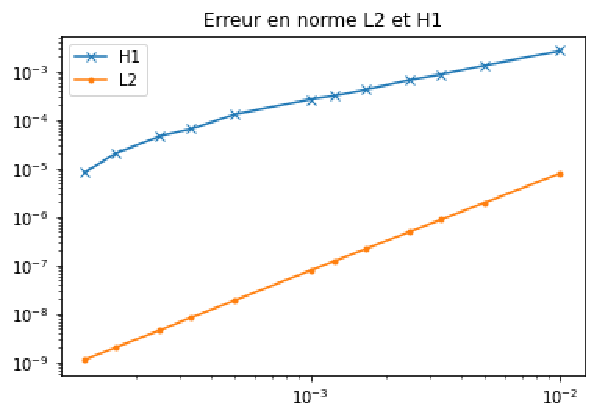
\includegraphics[scale=1]{erreurL2H1.pdf}
\caption[]{Résultat de l'étude de convergence }
\end{center}
\end{figure}




\begin{figure}
\begin{center}
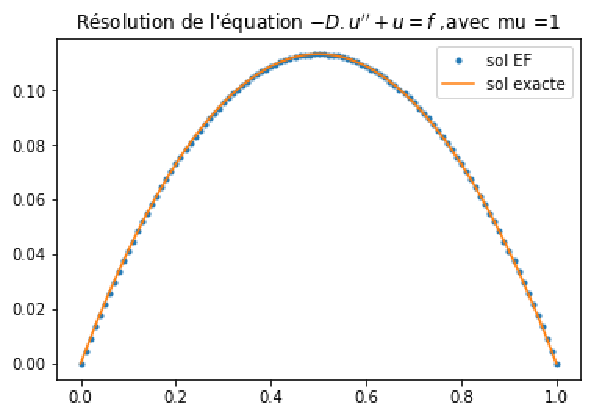
\includegraphics[scale=1]{sol_ef_exa.pdf}
\caption[]{Résolution de l'équation }
\end{center}
\end{figure}





\newpage


\section{Méthode des Bases reduites}



\subsection {Mise en oeuvre}
Posons 
$P_{0} = \{\mu_1,...,\mu_{N_0} \} \subset P \text{ , } V_{0}= vect(u_1,u_2,...,u_{N_0}) \text{ avec } u_i = u(\mu_i) \text{ et } V_{0} \subset  H_{0}^{1}.   \\
$
Ces fonctions $u_i$ sont obtenues en résolvant le problème approché par éléments
finis pour chaque $ \mu_i$ dans $P_{0}$.

Soit $ \mu \in P$ ,  On approche la fonction $u_{\mu}$ 
solution de base par une méthode de Galerkin dans 
$V_{0}$, ce qui revient à chercher la fonction 
$u^{BR}_{\mu} \in V_0$ telle que : 
$$
a_{\mu}(u^{BR}_{\mu},u_i) = b(u_i) , \forall i \in \{1,...,N_0\}
$$

En décomposant $u^{BR}_{\mu}$ sous la forme 
$u_{BR}^{\mu} = \sum_{i = 1}^{N_0} X^{BR}_{\mu,i}u_i$
et $u_i = \beta_1 \varphi_1 + ...+ \beta_N \varphi_N $

$
a_{\mu}(u^{BR}_{\mu},u_i) = \sum_{i= 1}^{N_0}
\sum_{k,j= 1}^{N} X^{BR}_{\mu,i} 
\beta_k \beta_j a_\mu(\varphi_{k},\varphi_{j}) \text{  car $a_{\mu}$ est billinéaire}
$


Posons
$$
X^{BR}_{\mu}  = \begin{pmatrix}
X^{BR}_{\mu,1} \\
. \\
. \\
. \\
X^{BR}_{\mu,N_0} \\
\end{pmatrix} , 
U = \begin{pmatrix}
u_1 , ... , u_{N_0}
\end{pmatrix} = \begin{pmatrix}
u_1 \\
. \\
. \\
. \\
u_{N_0} \\ 
\end{pmatrix}
$$


On   réécrit le système  :
$$
(U^{T}A_{\mu}U )X^{BR} = 
U^{T}(A_0 + M)U + \mu U^{T}A_1U = U^{T}B \\
$$
Notons $V_0 = U^{T}(A_0 + M)U$ ,  $V_1 = U^{T}A_1U$ et $B^{BR} = U^{T}B$ , $A^{BR}_{\mu} = V_0 + \mu V_1$.
Le problème s'écrit : $A^{BR}_{\mu} X^{BR} = B^{BR} $. 



\subsection {Algorithme glouton  }

Pour sélection les $N_0$ solutions de base , La procedure ci-dessous a été utilisé .



Pseudo-code de l'algorithme  :


    
\begin{tabbing}
\hspace{1cm} \= \hspace{1cm} \= \kill

choisir $\mu_1 $ de manière aléatoire \\
$u(\mu_1) = u_1$ \\
$B = Vect(u(\mu_1)$ \\
Pour i allant de 2 à ${N_0}$ faire :\\
\>    $u_i := \underset{\mu \in P}{argmax }(\Delta(B_i,\mu))$ \\
\>     $B_i := Vect(u_1,...,u_i)$
\end{tabbing}

$
\Delta(B,\mu) =|| u(\mu) - P_{B}u(\mu)||
$






\subsection{Etude du conditionnement ou sélection de la dimension}
Pour déterminer la valeur de optimale de $N_0$ , Nous avons calculer pour différent valeur de $N_0$, le condtionnement de la matrice 
U .

% ---- mettre image cond
\begin{figure}
\begin{center}
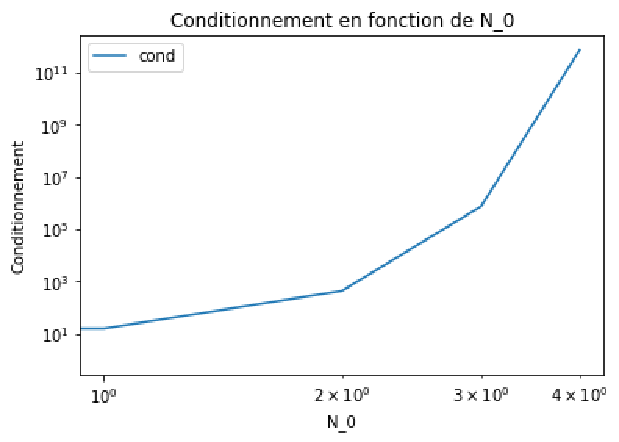
\includegraphics[scale=1]{cond.pdf}
\caption[]{Erreur en valeur absolu entre les solution EF et BR }
\end{center}
\end{figure}


\subsection{Qualité de la Base Reduite}

Pour différent valeur de M dans $\{ 10,100,500,1000,2000,2500,3000 \}$ , on calcul l'erreur entre la solution Ef et RB puis on affiche le graphe. 
$$
err = \underset{\Lambda ^{test}_{M}}{\sup} {||u^{EF}(\mu) - u^{RB}(\mu) ||_{L^{2}} }
$$

\begin{figure}
\begin{center}
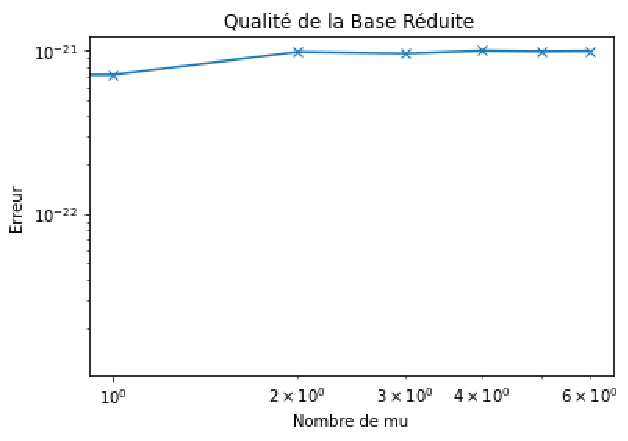
\includegraphics[scale=1]{qual_br.pdf}
\caption[]{Erreur en valeur absolu entre les solution EF et BR }
\end{center}
\end{figure}

\subsection{Etude de l'erreur }


\begin{figure}[h]
\begin{center}
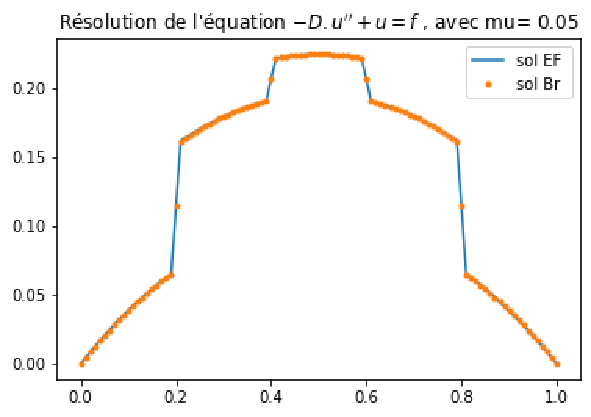
\includegraphics[scale=1]{sol_br_ef.pdf}
\caption[]{Résolution par les méthodes EF et BR }
\end{center}
\end{figure}

\begin{figure}[ht]
\begin{center}
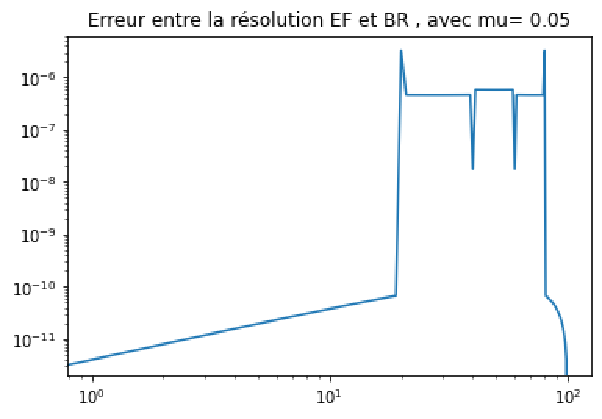
\includegraphics[scale=1]{err_br_ef.pdf}
\caption[]{Erreur en valeur absolu entre les solutions EF et BR }
\end{center}
\end{figure}


\newpage

\begin{thebibliography}{9}


\bibitem{Gianluigi Rozza}
Gianluigi Rozza,  \emph{An introduction to reduced basis method for parametrized PDEs
 }

\bibitem{B. Haasdonk}
B. Haasdonk,  \emph{Reduced Basis Methods for Parametrized PDEs –
A Tutorial Introduction for Stationary and
Instationary Problems }


\bibitem{Alexandre Ern}
Alexandre Ern,  \emph{ Analyse numérique et optimisation
Méthode des bases réduites }



\end{thebibliography}

\end{document}